\chapter{Bibliograf\'{\i}a por cap\'{\i}tulo y localizadores}
\label{C:cap2}

% Figuras de ESTE cap\'{\i}tulo + las compartidas.
\graphicspath{{figs/cap2/}{figs/comunes/}}

\section{Referencias repetidas entre cap\'{\i}tulos}
\label{S:repetidas}

Este cap\'{\i}tulo vuelve a citar trabajos que ya aparecieron en la
secci\'{o}n~\ref{S:citas}: \cite{Bohm1952PRp166} y \cite{Bohm1952PRp180}. En la
bibliograf\'{\i}a del final de este cap\'{\i}tulo van a aparecer de nuevo, y con otro
n\'{u}mero, porque cada cap\'{\i}tulo numera su lista desde 1. En el \texttt{.bib} la
entrada sigue existiendo una sola vez.

Esto lo hace la opci\'{o}n \verb|refsection=chapter| de biblatex, declarada en
\texttt{ibextra.sty}. Cada \verb|\chapter| abre una \emph{refsection} nueva y
\verb|\printbibliography| imprime s\'{o}lo la de la refsection en curso.

Tambi\'{e}n se puede citar algo que no apareci\'{o} antes, por ejemplo
\cite{Laricch2009AAMOP_ICBp3}, y mezclarlo con lo ya citado:
\cite{Bohm1952PRp166,Laricch2009AAMOP_ICBp3}.

\section{Las cuatro formas de citar una parte de un trabajo}
\label{S:localizadores}

\begin{description}
\item[P\'{a}gina] \verb|\cite[45]{clave}| $\rightarrow$ \cite[45]{Sakurai2011}.
  Al ser un n\'{u}mero solo, biblatex agrega el prefijo \'{e}l mismo.
\item[Rango de p\'{a}ginas] \verb|\cite[45-48]{clave}| $\rightarrow$
  \cite[45-48]{Sakurai2011}. Detecta el rango y pluraliza el prefijo.
\item[Cap\'{\i}tulo de un libro] \verb|\citecap{clave}{5}| $\rightarrow$
  \citecap{Sakurai2011}{5}. Equivale a \verb|\cite[cap.~5]{clave}|.
\item[Secci\'{o}n, ecuaci\'{o}n, figura] \verb|\citesec{clave}{5.3}| $\rightarrow$
  \citesec{Sakurai2011}{5.3}; \verb|\citeec{clave}{2.17}| $\rightarrow$
  \citeec{Sakurai2011}{2.17}; \verb|\citefig{clave}{3}| $\rightarrow$
  \citefig{Hunter07CSE}{3}.
\end{description}

Para texto arbitrario alcanza con poner el localizador completo a mano, por
ejemplo \verb|\cite[tomo II, ap. B]{clave}|, que da
\cite[tomo II, ap\'{e}ndice B]{Jackson1998}.

\section{Cuando la referencia ES un cap\'{\i}tulo de libro}
\label{S:inbook}

Hay dos casos distintos que conviene no mezclar:

\begin{enumerate}
\item \textbf{Cito un libro completo y se\~{n}alo d\'{o}nde mirar.} La entrada es
  \verb|@book| y el cap\'{\i}tulo va como localizador en la cita:
  \citecap{Sakurai2011}{5}.
\item \textbf{El cap\'{\i}tulo tiene autor propio y es la referencia en s\'{\i}.} La
  entrada es \verb|@incollection| (cap\'{\i}tulo con autor distinto del del libro,
  t\'{\i}pico en colecciones y reviews) o \verb|@inbook| (cap\'{\i}tulo del mismo autor
  del libro). Se cita normal, sin localizador:
  \cite{Briggs1991AAMOP_TTOp1} y \cite{Shankar1994Cap13}.
\end{enumerate}

\section{Una figura de la carpeta de este cap\'{\i}tulo}
\label{S:figura-cap2}

\begin{figure}[ht]
\centering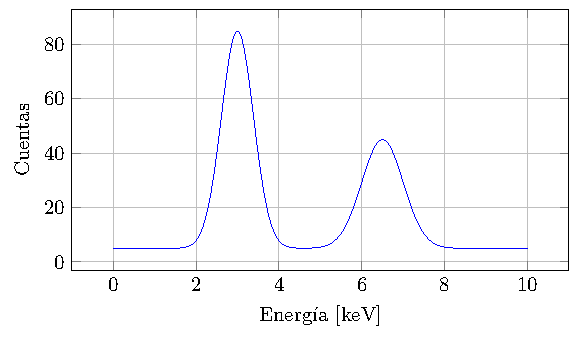
\includegraphics[width=\imsize]{cap2_espectro}
\caption[Espectro de ejemplo]{Esta figura est\'{a} en \texttt{figs/cap2/}. El
\texttt{\textbackslash includegraphics} no menciona la carpeta: la resuelve el
\texttt{\textbackslash graphicspath} del principio del archivo. Herramienta de
graficaci\'{o}n: \cite{Hunter07CSE}.\label{f:cap2-espectro}}
\end{figure}

% Bibliograf\'{\i}a de este cap\'{\i}tulo. Va al final del archivo, siempre.
\bibliografiacapitulo

%%% Local Variables:
%%% mode: latex
%%% TeX-master: "template"
%%% End:
